\chapter{Test Environment} \label{test}

Neste capítulo será abordada a configuração utilizada na implementação das ferramentas, assim como os procedimentos para os testar.

\section{Proxy}
Tal como no projeto anterior, o servidor de bancada funcionou como um proxy, de mode a que remotamente se tivesse acessos aos \textit{tux}s, nomeadamente aos sites gerados pelo \textbf{MRTG} e \textbf{NTOP}.
Esta configuração não será abordada neste relatório, dado que foi analisada no relatório anterior.

\section{Serviços}
Todos os serviços (Webmail, FTP, etc.) foram instalados no \textbf{tux12}. Note-se que no caso do NTP, foi preciso também instalar um cliente no \textbf{tux13}.
O mesmo se verifica no caso do Webmail, sendo que foi necessário a cooperação com colegas da sala I320, onde também foram instalados Webmail servers nesses computadores. 
A razão pela qual foi necessária esta cooperação deve-se ao princípio de funcionamento do MRTG (Capítulo \ref{prop_rede}).

O \textbf{NTOP} foi configurado no \textbf{tux12} e o \textbf{MRTG} no \textbf{tux13}.
O \textbf{tux14} não teve disponível na parte final do trabalho devido a erro durante a sua configuração que não pode ser corrigido presencialmente em tempo útil. Consequentemente, não foi utilizado.

\section{Routing}
Devido ao objetivo do trabalho, foi necessário fazer uso do router de bancada \textbf{rtr-1}.
O router de bancada está ligado à mesma rede local que os \textit{tux}s, através do switch, que por sua vez está ligado ao router de sala \textbf{firetux}.
Esta informação será util durante a utilização do MRTG.


\section{Cronjobs}
De forma similar ao projeto anterior, foram configurados \textit{cronjobs} para simular tráfego na rede. Este cronjobs estavam configurados: (Fig \ref{fig:crontab_1})
\begin{itemize}
    \item No \textit{tux12} e \textit{tux13}, para gerar tráfego local
    \item No \textit{gnu32}, para gerar tráfego não local que passasse pelo router
\end{itemize}

\begin{figure}
    \centering
    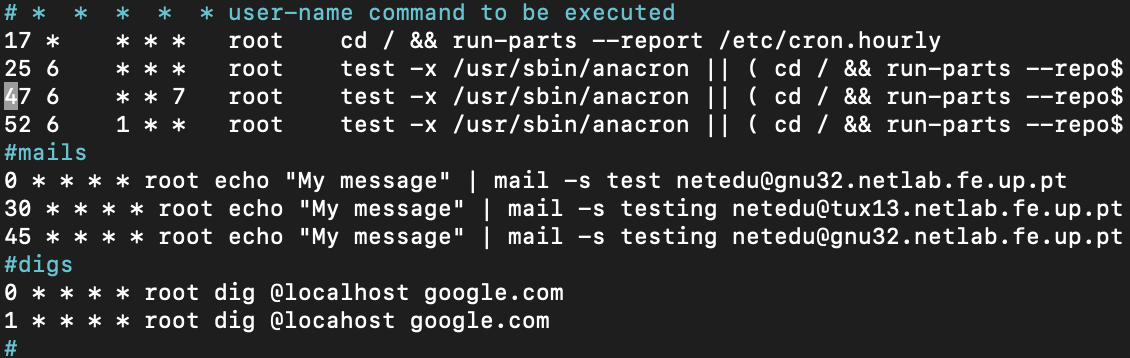
\includegraphics[width=.8\linewidth]{figs/setup/crontab_1.png}
    \caption{Exemplo dos Cronjobs no tux12}
    \label{fig:crontab_1}
\end{figure}

Este \textit{cronjobs} geram tráfego especifico de cada serviço nomeadamente:
\begin{itemize}
    \item SMTP (Simple Mail Transfer Protocol), ao enviar emails.
    \item FTP, ao fazer download de um ficheiro via FTP
    \item DNS, ao fazer queries, neste caso do \textit{google.com}
    \item HTTP, ao aceder ao sites através do \textit{wget}
\end{itemize}

O tráfego NTP é gerado automaticamente pois o computador sincroniza periodicamente com a hierarquia superior.



